\begin{apendicesenv}
\partapendices

\chapter{Termo de Abertura de Projeto}
\label{project_charter}

\begin{table}[h!]
\centering
\caption{Histórico de Versão}
\label{my-label}
\begin{tabular}{|l|l|l|l|}
\hline
\textbf{Data} & \textbf{Versão} & \textbf{Descrição}   & \textbf{Responsável} \\ \hline
24/03/2017    & 1.0             & Criação do Documento & Nicolas Boarin       \\ \hline
\end{tabular}
\end{table}

\section{Nome do Projeto}
Bicicleta Elétrica com Dispositivo de Auxílio à Rota

\section{Descrição do Projeto}
A proposta visa a criação de uma bicicleta elétrica com um sistema embarcado acoplado em sua estrutura. Este sistema embarcado quando sincronizado a um aplicativo de mapeamento GPS (que em parte será desenvolvido pelo grupo utilizando a API do Google Maps) irá mostrar ao ciclista com sinais visuais e tácteis a rota escolhida pelo mesmo no aplicativo, sem a necessidade de tirar o foco da estrada para verificar de forma contínua a rota pelo celular.

\section{Objetivos do Projeto}
Este projeto tem por objetivo uma redução do uso contínuo do celular, ao se usar um veículo (no caso abordado uma bicicleta elétrica),  a fim de um aumento da atenção do ciclista a sua rota desejada.

Dado o contexto no Brasil um dos objetivos secundários do projeto é que com a diminuição da frequência de uso do dispositivo móvel por um usuário do produto, isso poderá a diminuir as chances do mesmo poder a vir ser assaltado.

\textbf{Objetivos Gerais:}
\begin{itemize}
  \item Criação de uma bicicleta elétrica;
  \item Criação de um aplicativo para se “comunicar” com a bicicleta;
  \item Criação de um suporte na bicicleta para os componentes eletrônicos;
  \item Criação de um módulo de guia de rota GPS;
  \item Integração do módulo de guia no suporte da bicicleta e a sincronização com o app. 
\end{itemize}

\section{Justificativa do Projeto}
“As conversas de telefone celular tendem a restringir artificialmente a percepção periférica medida por um campo visual. Isso sugere que o uso do telefone celular durante a condução pode diminuir o campo visual perceptivo, tornando o condutor menos consciente do ambiente e mais suscetível a acidentes.” \cite{maples2008effects} 

	Tendo essas informações o projeto foi proposto a fim de reduzir a frequência de uso de um aparelho móvel enquanto o veículo elétrico estiver em movimento, assim aumentando a percepção do usuário ao seu redor, assim diminuindo o número de acidentes e respectivos assaltos causados por uma possível menor visibilidade do celular.

\section{Recursos do Projeto}
A solução proposta possui os seguintes recursos:
\begin{itemize}
	\item Aplicativo para dispositivo móvel de escolha a rota GPS;
	\item Sistema de retroalimentação de energia por pedaladas;
	\item Módulo de luzes guias para a rota selecionada;
	\item Motor e controladores instalados na bicicleta.
\end{itemize}

\section{Subprodutos Identificados}
A solução apresentada possui os seguintes subprodutos:

\begin{itemize}
	\item Aplicação de Dashboard Interativa - O aplicativo criado pelo grupo possuirá como funcionalidade principal a escolha da rota, mas também contará com funções como uma dashboard de acompanhamento das viagens do usuário com métricas como "Km percorridos" e "Tempo gasto por rota".
	\item Estrutura Física da Bicicleta - A bicicleta será projetada a fim de manter o centro de massa no centro, sua estrutura também será designada a ponto de tentar maximizar a vida útil de todos os componentes eletroeletrônicos de riscos como vibração, temperatura e exposição ao Sol. 
\end{itemize}

\section{Stakeholders}
Qualquer tipo de pessoa que seja envolvida no projeto de alguma forma, seja no próprio desenvolvimento, no auxílio, ou mesmo uso do produto final foram considerados stakeholders.  A tabela abaixo mostra os stakeholders identificados pelo grupo:

\begin{table}[h!]
\centering
\caption{Stakeholders}
\label{my-label}
\begin{tabular}{|lll|}
\hline
\multicolumn{1}{|l|}{\textbf{Nome}} & \multicolumn{1}{l|}{\textbf{Descrição}}               & \textbf{Responsabilidades}                                             \\ \hline
Integrantes do Projeto              & Integrantes do grupo de desenvolvimento do projeto    & Produzir, analisar, verificar, acoplar módulos e validar produto final \\
Professores de PI2                  & Professores da disciplina de PI2                      & Verificar o andamento do projeto e auxiliar e por fim avaliar o mesmo  \\
Usuários de Teste                   & Pessoas que utilizarão os protótipos feito pelo grupo & Utilizar o protótipo a fim de dar feedback sobre possíveis melhorias   \\
Usuários Finais                     & Pessoas que utilizarão o produto final                & Usufruir do projeto em seu dia a dia                                   \\ \hline
\end{tabular}
\end{table}


\section{Líderes do Projeto e Suas Responsabilidades}
Sendo um projeto integrador, cada engenharia terá até uma certa parte seu trabalho feito de forma que cada frente de uma determinada engenharia possua autonomia. Cada um dos grupos de uma engenharia específica possuirão um representante para se comunicar com outros líderes. 

Os líderes ficam responsáveis pela área de gerenciamento e auxílio de cada time que ele está encarregado e também como representante de sua área caso outro grupo possua uma dependência da área na qual o mesmo atua. 

Após as escolhas dos devidos líderes a lista atualizada de líderes e suas áreas é:

\begin{itemize}
	\item Frente Estrutural/Mecânica - Marlos Pereira
	\item Frente Eletromecânica - Rodrigo Araújo
	\item Frente Eletroeletrônica - Bruno Fares
	\item Frente Software - Levi Moraes
	\item Frente Energia/Alimentação - Karine Ximenes
\end{itemize}

\section{Cronograma de marcos sumarizado}
Os principais marcos do projeto, juntos com suas descrições e respectivos responsáveis foram detalhados  na tabela abaixo:  

\begin{table}[]
\centering
\caption{Macro Cronograma}
\label{my-label}
\begin{tabular}{|l|l|l|}
\hline
\textbf{Data}         & \textbf{Marcos}                                                                    & \textbf{Descrição}                                                                                                                                                                                                                                        \\ \hline
17/03/17              & \begin{tabular}[c]{@{}l@{}}Proposta Inicial\\ e Formação do Grupo\end{tabular}     & \begin{tabular}[c]{@{}l@{}}Definição em aula sobre a ideia do projeto\\ de forma abstrata junto com os integrantes que irão compor o grupo\end{tabular}                                                                                                   \\ \hline
18/03 $\sim$ 24/03/17 & Refinamento da proposta                                                            & \begin{tabular}[c]{@{}l@{}}Reuniões entre o grupo para criar uma visão\\ compartilhada sobre o projeto\end{tabular}                                                                                                                                       \\ \hline
05/04 $\sim$ 07/04/17 & Ponto de Controle 1                                                                & \begin{tabular}[c]{@{}l@{}}Apresentação do grupo sobre a concepção do projeto,\\ já com a ideia bem definida sobre o escopo do mesmo\\ e requisitos bem refinados, a fim de mostrar o que será\\ desenvolvido no projeto para os professores\end{tabular} \\ \hline
08/04 $\sim$ 25/05/17 & Criação dos Módulos Específicos                                                    & \begin{tabular}[c]{@{}l@{}}Cada grupo ficará encarregado da criação de\\ seus respectivos módulos/componentes\end{tabular}                                                                                                                                \\ \hline
31/05 $\sim$ 02/06/17 & Ponto de Controle 2                                                                & \begin{tabular}[c]{@{}l@{}}Apresentação dos componentes de cada engenharia\\ para a banca avaliadora junto com o andamento do projeto\end{tabular}                                                                                                        \\ \hline
04/06 $\sim$,29/06/17 & \begin{tabular}[c]{@{}l@{}}Integração de Componentes e \\ Homologação\end{tabular} & \begin{tabular}[c]{@{}l@{}}Integração dos módulos de cada engenharia a fim\\ de entregar o produto final com todos seus respectivos teste\end{tabular}                                                                                                    \\ \hline
05/07/17              & Ponto de Controle 3                                                                & \begin{tabular}[c]{@{}l@{}}Apresentação do produto final para a bancada avaliadora, \\ mostrando os respectivos testes definidos de acordo com os requisitos definidos pelo grupo.\end{tabular}                                                           \\ \hline
\end{tabular}
\end{table}

\section{Investimento Preliminar}
Como ainda não foi definida uma estrutura ideal para o projeto, uma estimativa precisa sobre o preço não pode ser dada, mas o grupo avaliou que para um investimento inicial cada integrante teria teria que entrar com R\$ 100,00, tirando o motor elétrico que um integrante já possuía (estimado em R\$ 500,00), então o valor preliminar foi definido como R\$ 1.800,00.

\section{Restrições e Riscos}
Os riscos inicialmente apontados pela equipe para o projeto em questão estão listados na tabela abaixo. Junto com o nome do risco também estão definidas as respostas, causas,  probabilidades, severidades e prioridades de cada um:

\begin{table}[h!]
\centering
\caption{Riscos}
\label{my-label}
\begin{tabular}{|llllll|}
\hline
\multicolumn{1}{|l|}{\textbf{Risco}}                                 & \multicolumn{1}{l|}{\textbf{Resposta}}                        & \multicolumn{1}{l|}{\textbf{Causas}}                                                 & \multicolumn{1}{l|}{\textbf{Probabilidade}} & \multicolumn{1}{l|}{\textbf{Severidade}} & \textbf{Prioridade} \\ \hline
Trancamento de um integrante do grupo                                & Redistribuir as atividades entre os membros da mesma equipe   & Problemas Pessoais                                                                   & Remoto                                      & Moderado                                 & Monitorar           \\
Atraso nas entregas das atividadesAtraso nas entregas das atividades & Realinhar o cronograma e atuação do responsável por tal grupo & Problemas acadêmicos                                                                 & Provável                                    & Significante                             & Ação Urgente        \\
Desentendimento entre os membros da equipe                           & Alinhamento de idéias através dos líderes                     & Idéias divergentes                                                                   & Ocasional                                   & Baixo                                    & Monitorar           \\
Atraso na entrega de um produto/serviço                              & Reunião dos líderes e tomada de ação no setor com problemas   & Problema de comunicação entre os representantes e os outros integrantes de seu grupo & Ocasional                                   & Significante                             & Ação Urgente        \\
Problemas com a API                                                  & Procurar uma nova API                                         & Limitação da própria API                                                             & Remoto                                      & Catastrófico                             & Ação Urgente        \\
Vibração do motor                                                    & Procurar uma solução melhor                                   & Problemas Estruturais                                                                & Remoto                                      & Baixo                                    & Monitorar           \\
Aquecimento dos componentes                                          & Replanejamento da estrutura                                   & Mal planejamento da estrutura                                                        & Remoto                                      & Moderado                                 & Monitorar           \\
Ergonomia do produto                                                 & Replanejamento Estrutural                                     &                                                                                      & Remoto                                      & Baixo                                    & Monitorar           \\
Custo inviável                                                       & Replanejamento dos componentes                                & Custo elevado dos componentes                                                        & Remoto                                      & Significante                             & Monitorar           \\ \hline
\end{tabular}
\end{table}

\chapter{Lista é Não é}


\chapter{Plano de Gerenciamento}
\chapter{Plano de RH}
	
	\chapter{Plano de Riscos}
\subsection{Objetivos}
	Este documento tem como finalidade estabelecer um processo de gerenciamento de riscos que podem vir a acontecer no projeto e a identificação dos mesmos pela equipe.

	\subsection{Descrição dos processos de gerenciamento de riscos}
	O Plano de Gerenciamento de Riscos contém seus processos definidos em quatro abordagens específicas segundo Max \cite{wideman1992project}. Sendo que todas as abordagens são necessárias pois elas se complementam para gerenciamento todas elas foram adotadas, sendo elas:
	
		\graphicspath{{figuras/}}
		\begin{figure}[h]
		\centering
		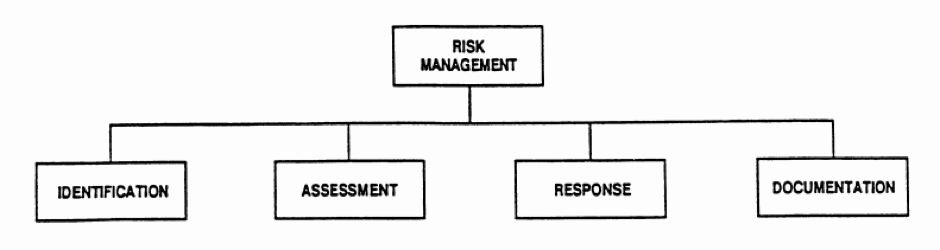
\includegraphics[scale=0.80]{EAP_Gerenciamento_de_Riscos.png}
		\caption{Etapas do plano de gerenciamento de riscos segundo Max \cite{wideman1992project}}
		\label{img:eap_gerenciamento_de_risco}
		\end{figure}
	
	\begin{itemize}
	 \item \textbf{Identificação}: Esta fase consiste em identificar todos os possíveis riscos que podem impactar de forma severa o sucesso do projeto. Os tipos de impacto podem variar dependendo de onde ele afeta no projeto e quais as probabilidades deles acontecerem. Combinações de riscos que juntos podem representar uma ameaça mais do que individualmente não podem ser ignorados.
	 \item \textbf{Avaliação}: Tendo identificado todo o alcance de riscos possíveis o próximo passo é os avaliar. O propósito é determinar os atributos do erro como o impacto, probabilidade e tipo de erro.
	\item \textbf{Resposta}: A parte de mitigação de riscos no projeto consiste em estabelecer uma estratégia de sistema apropriada, assim garantindo uma abordagem apropriada aos riscos caso eles venham a acontecer. Nesta etapa é descrito qual será a reação da equipe para tratar algum tipo de risco caso ele venha a acontecer.
	\item \textbf{Documentação}: Documento final e vital para o projeto que detalha todos os riscos, com suas características e quais serão as ações tomadas pela equipe de forma detalhada,caso cada risco apontado chegue a acontecer.
	\end{itemize}

	\subsection{EAR - Estrutura Analítica de Riscos para identificação dos riscos}
	O Project Management Institute (PMI), instituto que elaborou o Project Management Book of Knowledge (PMBoK) \cite{pmbok2012}, possui um template de estrutura analitica de riscos que possui as seguintes categorias e sub-divisões: 
	
	\graphicspath{{figuras/}}
	\begin{figure}[h!]
	\centering
	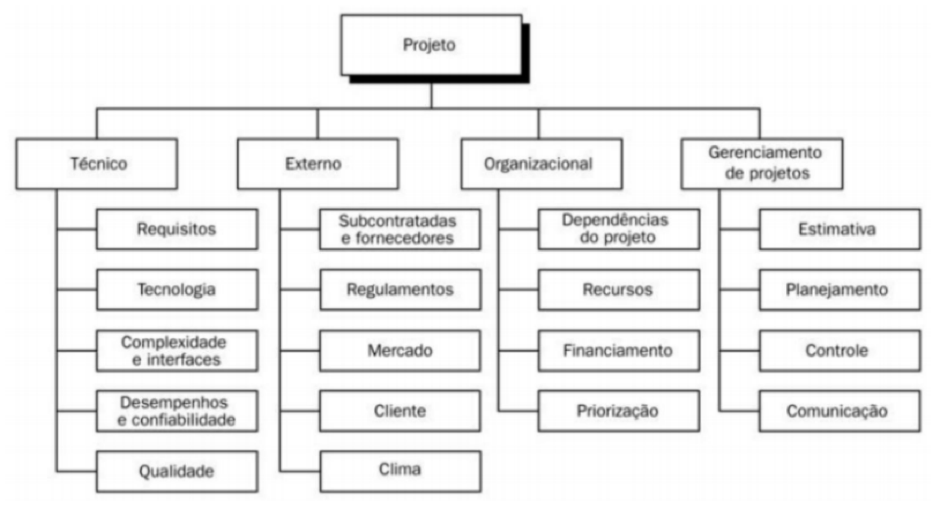
\includegraphics[scale=0.80]{classificacao_de_riscos.png}
	\caption{Classificação dos riscos na EAR segundo o PMI}
	\label{img:classificacao_de_riscos}
	\end{figure}
	
	\graphicspath{{figuras/}}
	\begin{figure}[h!]
	\centering
	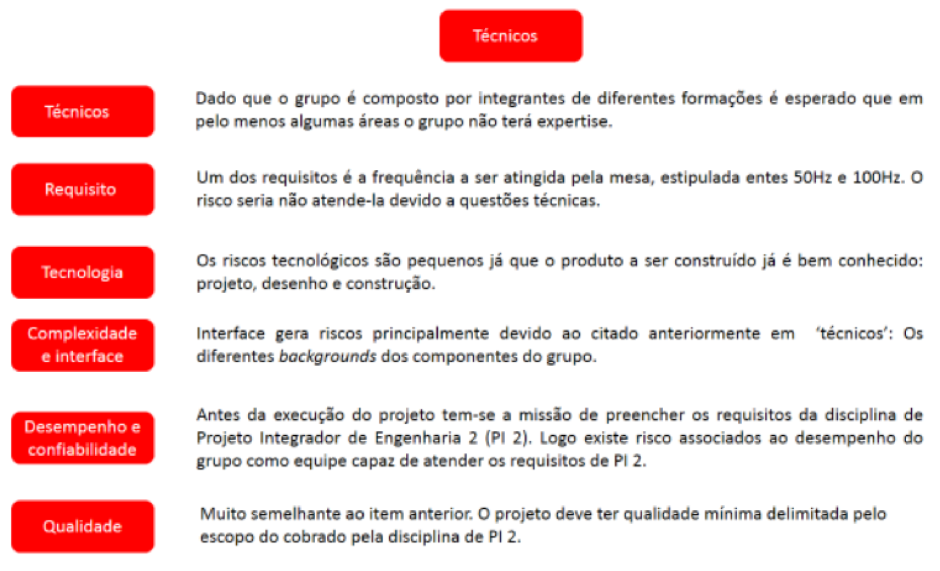
\includegraphics[scale=0.80]{analise_riscos_tecnicos.png}
	\caption{Análise em relação aos riscos técnicos}
	\label{img:analise_riscos_tecnicos}
	\end{figure}
	
	\graphicspath{{figuras/}}
	\begin{figure}[h!]
	\centering
	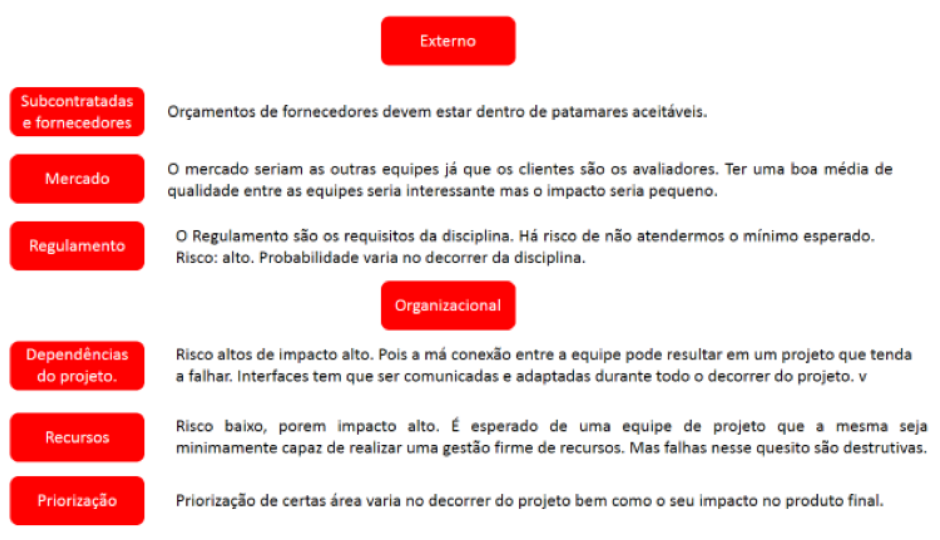
\includegraphics[scale=0.80]{analise_riscos_externos.png}
	\caption{Análise em relação aos riscos externos e organizacionais}
	\label{img:analise_riscos_externos}
	\end{figure}	
	
	\subsection{Qualificação dos Riscos}
	Os riscos identificados pelo grupo foram qualificados de acordo com sua probabilidade de ocorrência e o impacto resultante no projeto. O sistema de probabilidade e impactos foram classificados de acordo com a tabela padronizada do Gantter (ferramenta de gerenciamento de riscos adotada pela equipe).
	
	\begin{table}[h!]
\centering
\caption{Probabilidade dos Riscos}
\label{tabela_probabilidade_riscos}
\begin{tabular}{|ll|}
\hline
\multicolumn{1}{|l|}{\textbf{Nível}} & \textbf{Probabilidade} \\ \hline
Improvável                           & 0\% $\sim$ 20\%        \\
Remoto                               & 21\% $\sim$ 40\%       \\
Ocasional                            & 41\% $\sim$ 60\%       \\
Provável                             & 61\% $\sim$ 80\%       \\
Frequente                            & 81\% $\sim$ 100\%      \\ \hline
\end{tabular}
\end{table}	

\begin{table}[h!]
\centering
\caption{Severidade dos Riscos}
\label{tabela_severidade_de_riscos}
\begin{tabular}{|ll|}
\hline
\multicolumn{1}{|l|}{\textbf{Nível}} & \textbf{Descrição}                                                                                                                                                             \\ \hline
Negligível                           & Risco que não afeta a integridade do projeto de forma a comprometer o mesmo.                                                                                                   \\ \hline
Baixo                                & Possui pouco prejuízo ao desenvolvimento do projeto.                                                                                                                           \\ \hline
Moderado                             & \begin{tabular}[c]{@{}l@{}}Prejudica o desenvolvimento do projeto. Pode ser resolvido\\ em um curto período de tempo.\end{tabular}                                             \\ \hline
Significante                         & \begin{tabular}[c]{@{}l@{}}Prejudica o desenvolvimento do projeto. Gasta-se um tempo significativo\\ (semanas) para conseguir restituir a integridade do projeto.\end{tabular} \\ \hline
Catastrófico                         & Erro que previne o projeto de ser concluído.                                                                                                                                   \\ \hline
\end{tabular}
\end{table}
	
	\subsection{Prioridade dos Riscos}
	A prioridade dos riscos também foi feita de acordo com as opções já padronizadas da ferramenta “Gantter”, sendo elas:
	
	\begin{table}[h!]
\centering
\caption{Prioridade dos Riscos}
\label{tabela_prioridade_dos_riscos}
\begin{tabular}{|ll|}
\hline
\multicolumn{1}{|l|}{\textbf{Nível}} & \textbf{Descrição}                                                                                                                                                                                                                  \\ \hline
Sem Ação                             & O risco é tão pequeno ou irrelevante que nenhuma ação será tomada.                                                                                                                                                                  \\ \hline
Monitorar                            & \begin{tabular}[c]{@{}l@{}}O risco possui um certo grau de causar problemas, sendo \\ monitorado constantemente.\end{tabular}                                                                                                       \\ \hline
Tomar Ação                           & \begin{tabular}[c]{@{}l@{}}O risco possui uma boa probabilidade de causar problemas no projeto \\ e devem ser tomadas medidas de mitigação para que o mesmo não \\ aconteça ou reduza seu impacto.\end{tabular}                     \\ \hline
Ação Urgente                         & \begin{tabular}[c]{@{}l@{}}O risco possui uma boa probabilidade de causar muitos problemas no \\ projeto e devem ser tomadas medidas prioritárias de mitigação para que\\  o mesmo não aconteça ou reduza seu impacto.\end{tabular} \\ \hline
Interromper Projeto                  & \begin{tabular}[c]{@{}l@{}}O risco é tão significante que se interrompe o projeto até que seja \\ encontrada uma forma de contornar tal erro.\end{tabular}                                                                          \\ \hline
\end{tabular}
\end{table}	
	
	\subsection{Riscos Identificados}
	Os riscos identificados para o projeto estão listados na Tabela \ref{riscos_identificados}

\begin{table}[h!]
\centering
\caption{Riscos Identificados}
\label{riscos_identificados}
\begin{tabular}{|llll|}
\hline
\multicolumn{1}{|l|}{\textbf{Risco}}       & \multicolumn{1}{l|}{\textbf{Probabilidade}} & \multicolumn{1}{l|}{\textbf{Severidade}} & \textbf{Prioridade} \\ \hline
Trancamento de um integrante do grupo      & Remoto                                      & Moderada                                 & Monitorar           \\ \hline
Atraso nas entregas das atividades         & Provável                                    & Significante                             & Ação Urgente        \\ \hline
Desentendimento entre os membros da equipe & Ocasional                                   & Baixa                                    & Monitorar           \\ \hline
Atraso na entrega de um produto/serviço    & Ocasional                                   & Significante                             & Ação Urgente        \\ \hline
Problemas com a API                        & Remoto                                      & Catastrófica                             & Ação Urgente        \\ \hline
Vibração do motor                          & Remoto                                      & Baixa                                    & Monitorar           \\ \hline
Aquecimento dos componentes                & Remoto                                      & Moderada                                 & Monitorar           \\ \hline
Ergonomia do produto                       & Remoto                                      & Baixa                                    & Monitorar           \\ \hline
Custo inviável                             & Remoto                                      & Significante                             & Monitorar           \\ \hline
Atraso/falta dos integrantes nas reuniões  & Remoto                                      & Moderada                                 & Tomar Ação          \\ \hline
\end{tabular}
\end{table}

	\subsection{Ação de Resposta aos Riscos}
	As ações que foram definidas pelo time à serem tomadas para cada risco identificado se encontram na Tabela \ref{acoes_de_resposta}.

\begin{table}[!h]
\centering
\caption{Ações de Respostas aos Riscos}
\label{acoes_de_resposta}
\begin{tabular}{|ll|}
\hline
\multicolumn{1}{|l|}{\textbf{Risco}}       & \textbf{Resposta}                                                                                        \\ \hline
Trancamento de um integrante do grupo      & \begin{tabular}[c]{@{}l@{}}Redistribuir as atividades entre os \\ membros da mesma equipe\end{tabular}   \\ \hline
Atraso nas entregas das atividades         & \begin{tabular}[c]{@{}l@{}}Realinhar o cronograma e atuação do \\ responsável por tal grupo\end{tabular} \\ \hline
Desentendimento entre os membros da equipe & Alinhamento de idéias através dos líderes                                                                \\ \hline
Atraso na entrega de um produto/serviço    & \begin{tabular}[c]{@{}l@{}}Reunião dos líderes e tomada de ação no \\ setor com problemas\end{tabular}   \\ \hline
Problemas com a API                        & Procurar uma nova API                                                                                    \\ \hline
Vibração do motor                          & Procurar uma solução melhor                                                                              \\ \hline
Aquecimento dos componentes                & Replanejamento da estrutura                                                                              \\ \hline
Ergonomia do produto                       & Replanejamento da estrutura                                                                              \\ \hline
Custo inviável                             & Replanejamento dos componentes                                                                           \\ \hline
Atraso/falta dos integrantes nas reuniões  & \begin{tabular}[c]{@{}l@{}}Comunicação entre os representantes do \\ grupo com o indivíduo\end{tabular}  \\ \hline
\end{tabular}
\end{table}
	
	\subsection{Sistema de Controle de Mudanças de Riscos}
	O sistema serve justamente para alinhar a equipe sobre os riscos que o projeto pode vir a ter em seu decorrer e quais serão as ações que devem ser tomadas para cada tipo. A equipe deve estar consciente da probabilidade de cada risco encontrado a fim de controlar e manter o progresso do projeto em um meio que o risco possa sempre ser evitado.

	Cada risco não encontrado pelo grupo na fase de elaboração do projeto deverá ser documentado neste documento no futuro segundo os padrões adotados pela equipe e da ferramenta usada por ela para gerenciamento de riscos.
	
	
	\subsection{Plano de Custos}
	
	\subsection{Plano de Aquisições}
	
	\subsection{Cronograma Detalhado}
\label{schedule_ap}

Para evitar poluição visual no relatório, foram feitas duas versões do cronograma.
Dentro do relatório foi incluída uma versão simplificado do mesmo, sem o detalhamento de todas as atividades.
As figuras seguintes mostram o cronograma detalhado.

\begin{figure}[!htbp]
  \centering
  \includegraphics[width=\textwidth]{figuras/cronograma_det_1.eps}
  \caption{Cronograma de Atividades detalhado (parte 1). Fonte: autores.}
  \label{fig:cron_d1}
\end{figure}

\vfill
\pagebreak

\begin{figure}[!htbp]
  \centering
  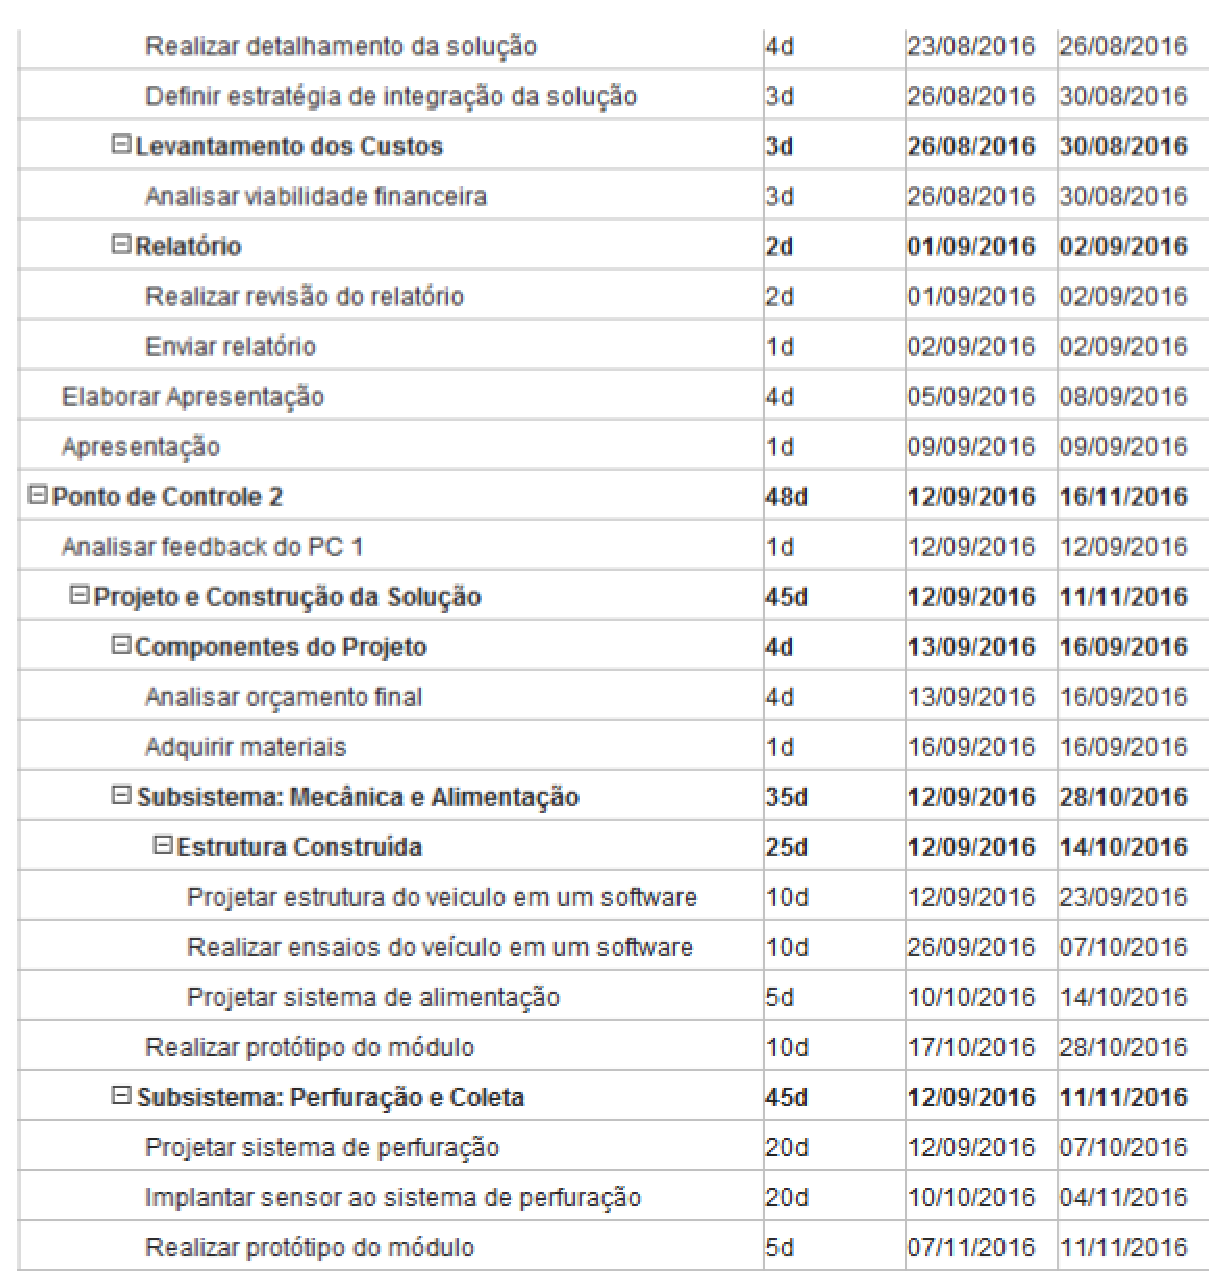
\includegraphics[width=\textwidth]{figuras/cronograma_det_2.eps}
  \caption{Cronograma de Atividades detalhado (parte 2). Fonte: autores.}
  \label{fig:cron_d2}
\end{figure}

\vfill
\pagebreak

\begin{figure}[!htbp]
  \centering
  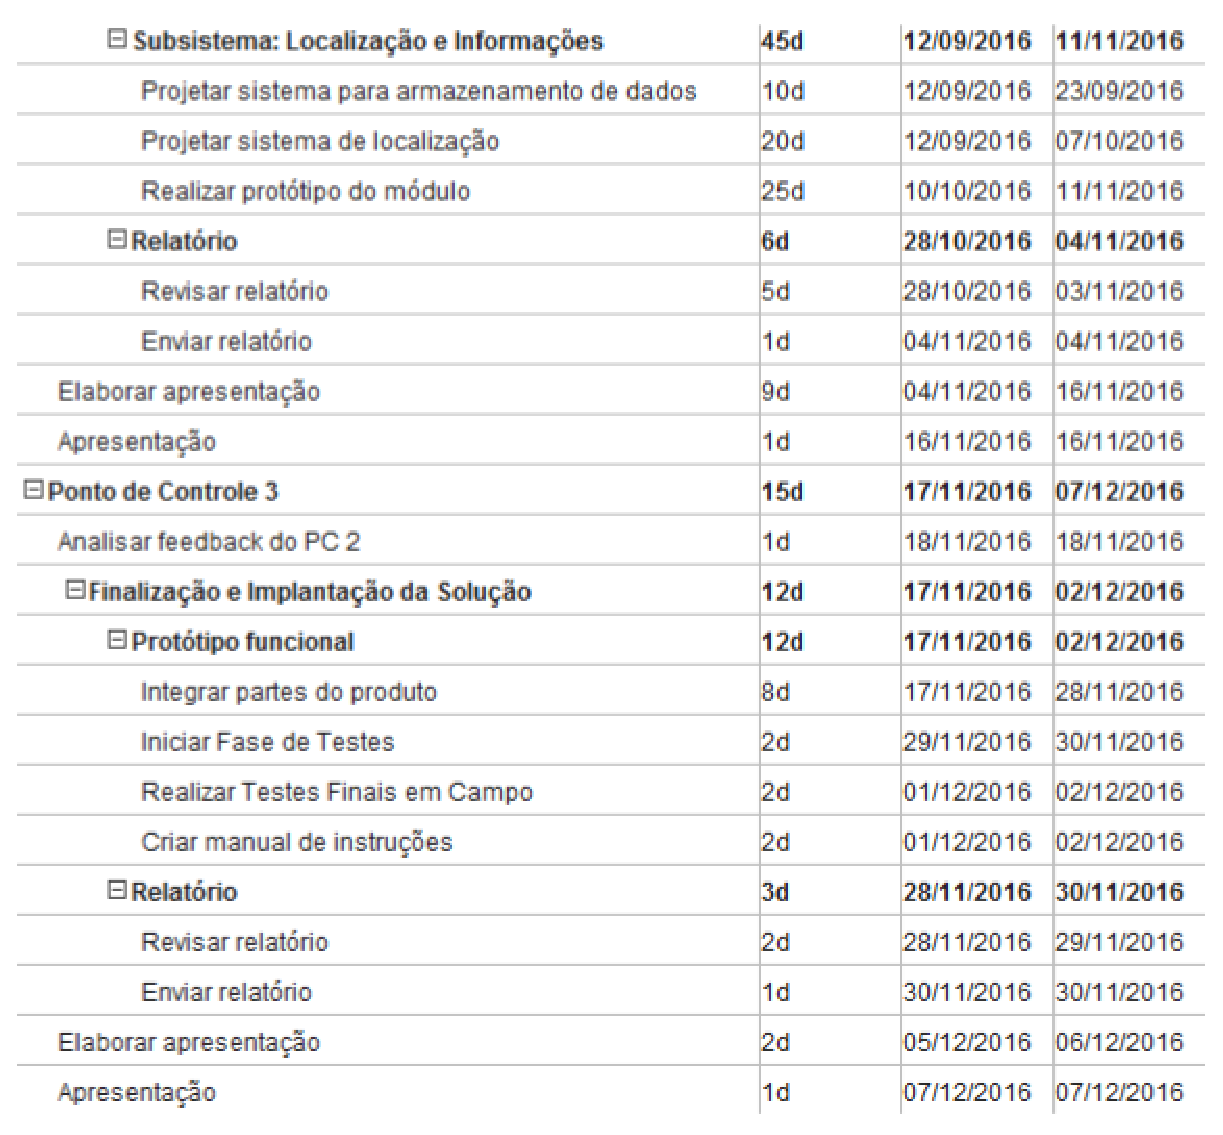
\includegraphics[width=\textwidth]{figuras/cronograma_det_3.eps}
  \caption{Cronograma de Atividades detalhado (parte 3). Fonte: autores.}
  \label{fig:cron_d3}
\end{figure}

\chapter{Desenhos Técnicos da Estrutura}

\begin{figure}[!htbp]
	\centering
	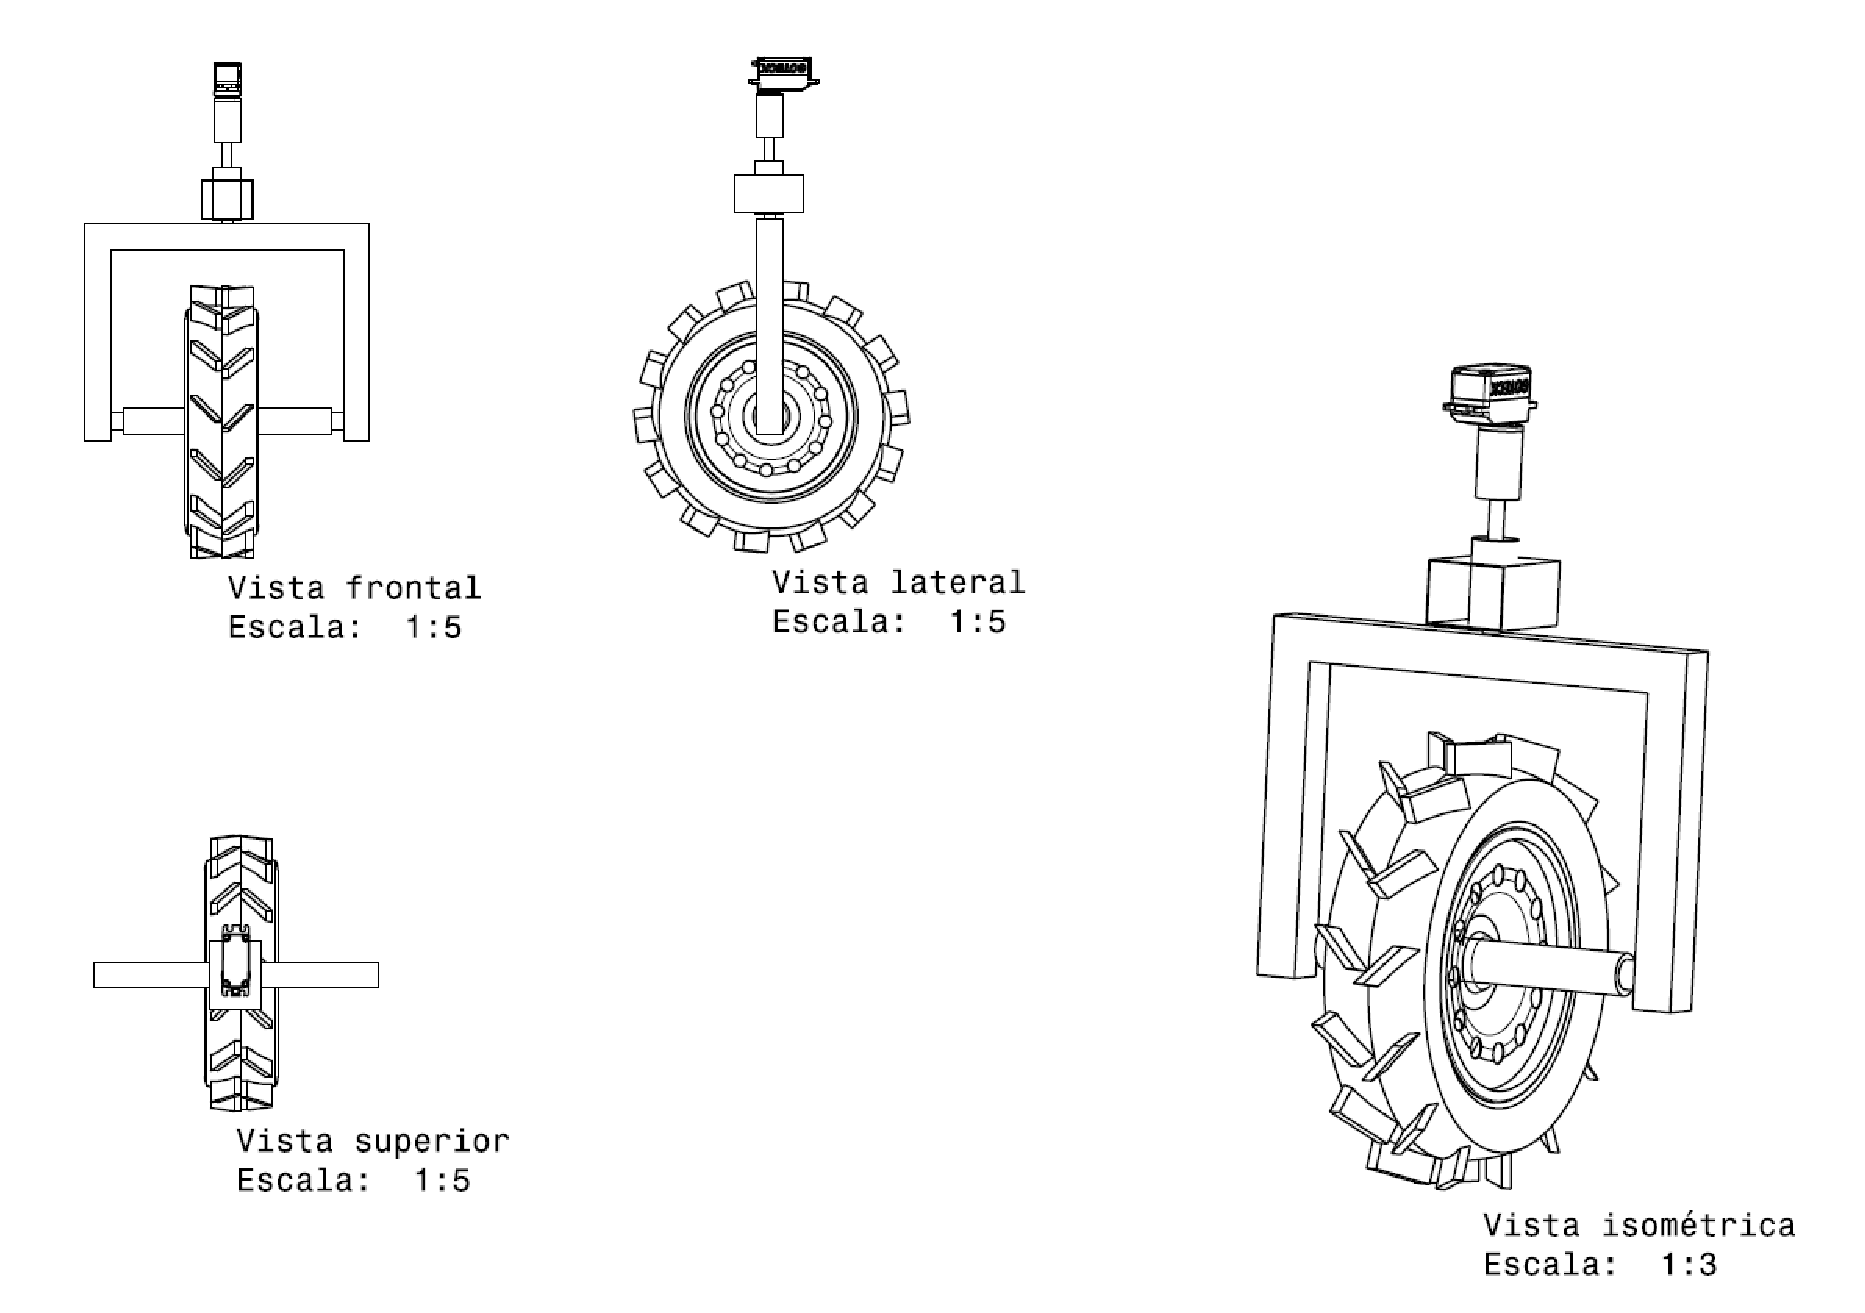
\includegraphics[width=\textwidth]{figuras/dt_direcao1.eps}
	\caption{Vistas frontal, lateral e superior da estrutura da direção}
\end{figure}

\begin{figure}[!htbp]
	\centering
	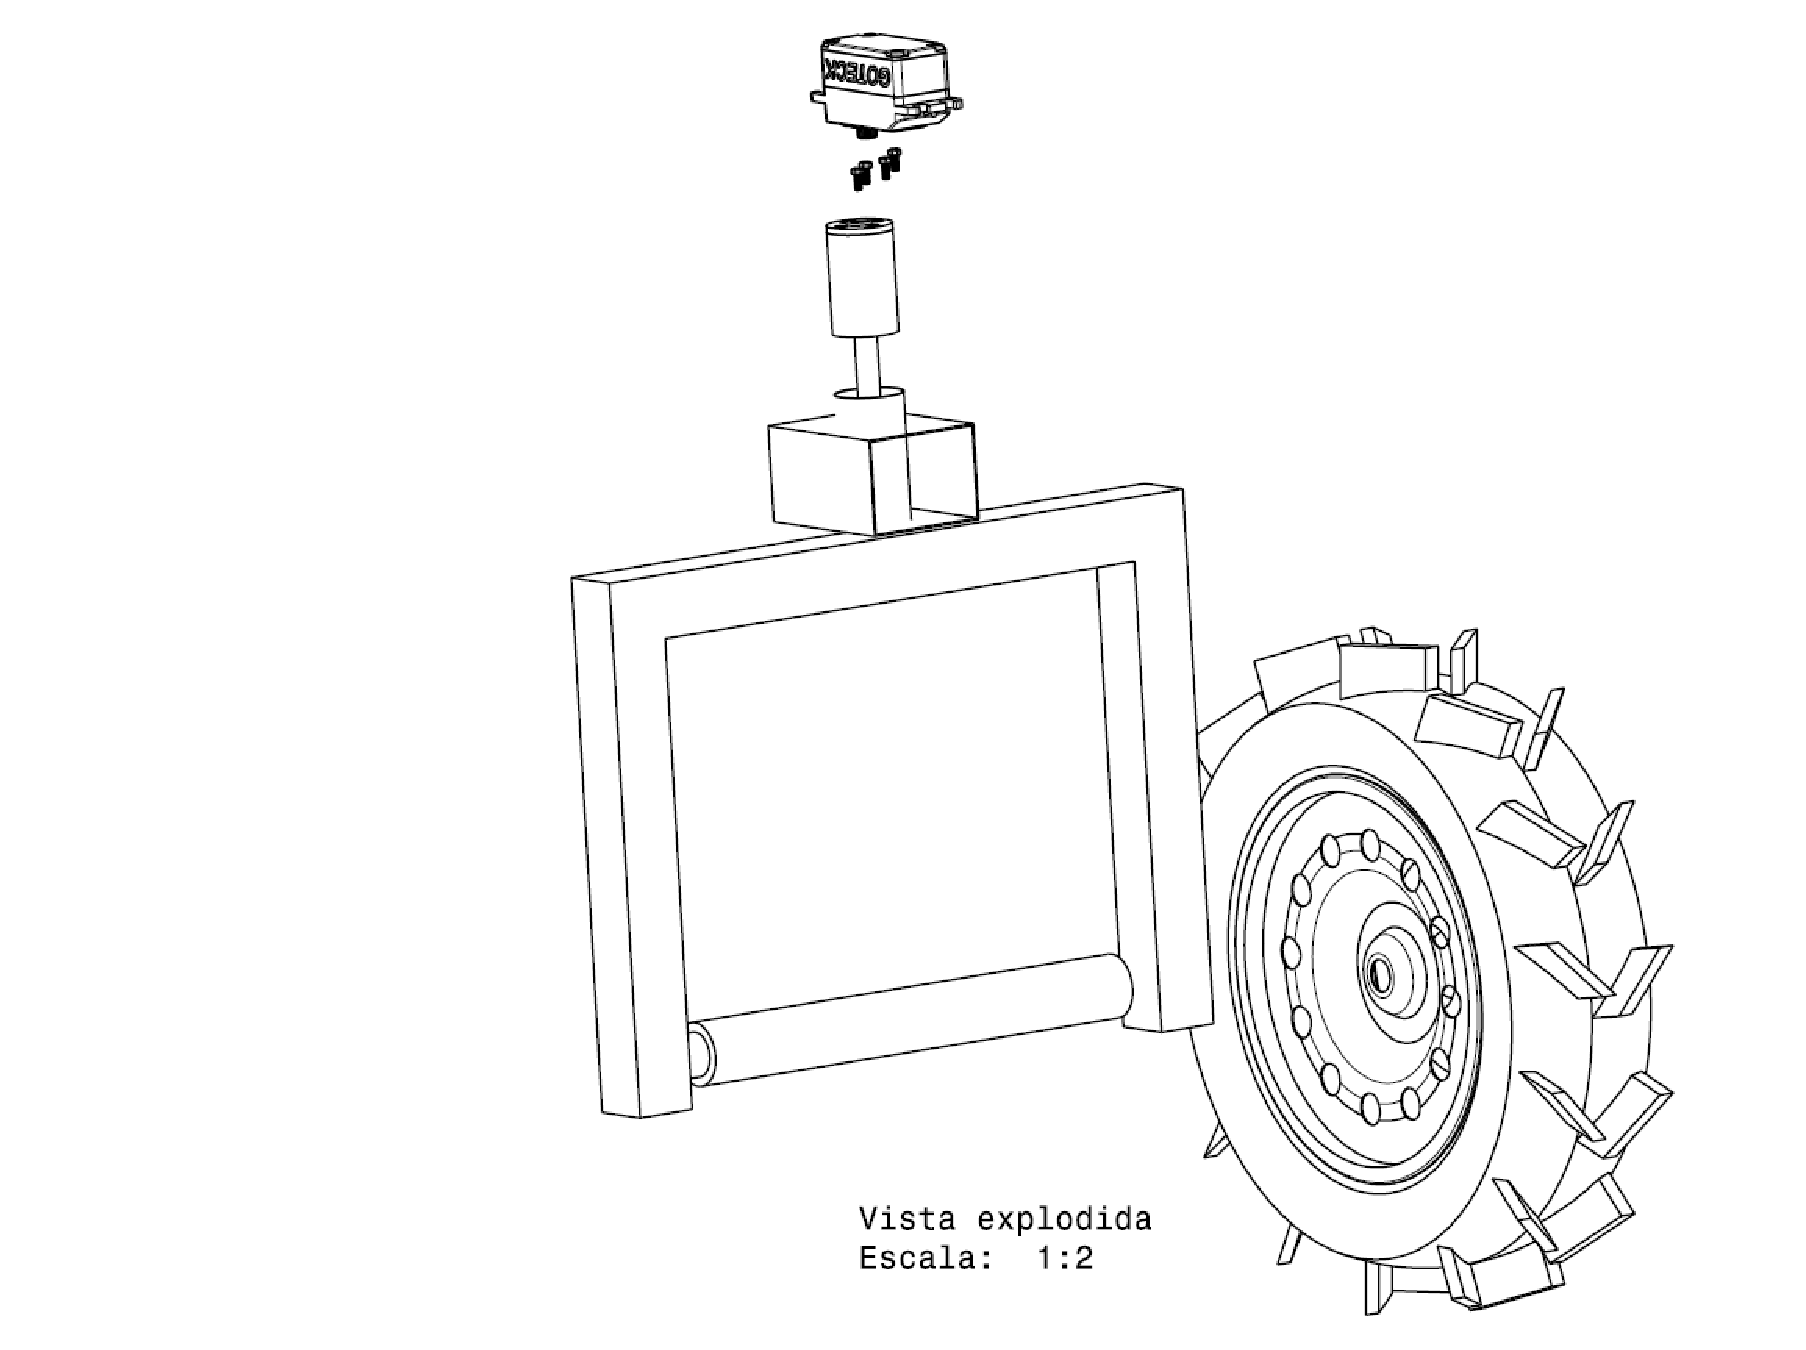
\includegraphics[width=\textwidth]{figuras/dt_direcao2.eps}
	\caption{Vista explodida do sistema de direção}
\end{figure}

\begin{figure}[!htbp]
	\centering
	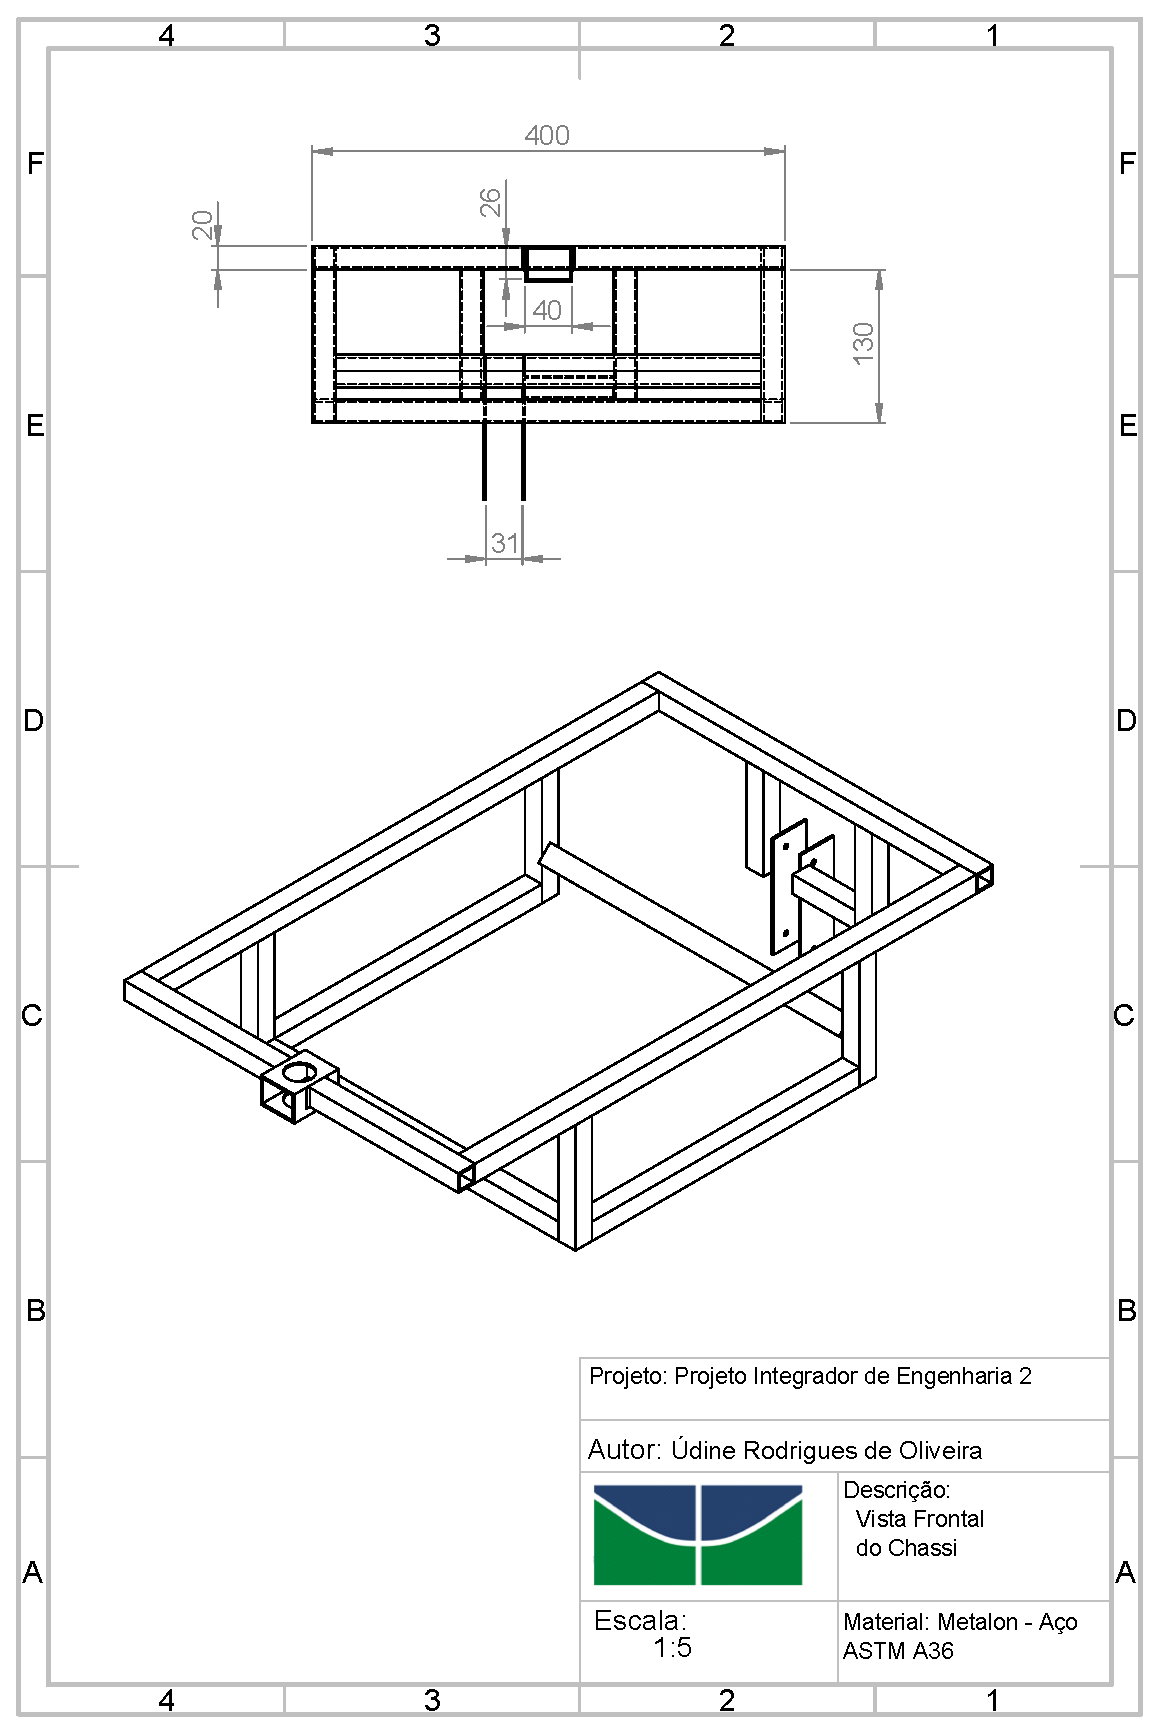
\includegraphics[width=\textwidth]{figuras/chassi_frontal.eps}
	\caption{Desenho técnico da vista frontal do chassi}
\end{figure}

\begin{figure}[!htbp]
	\centering
	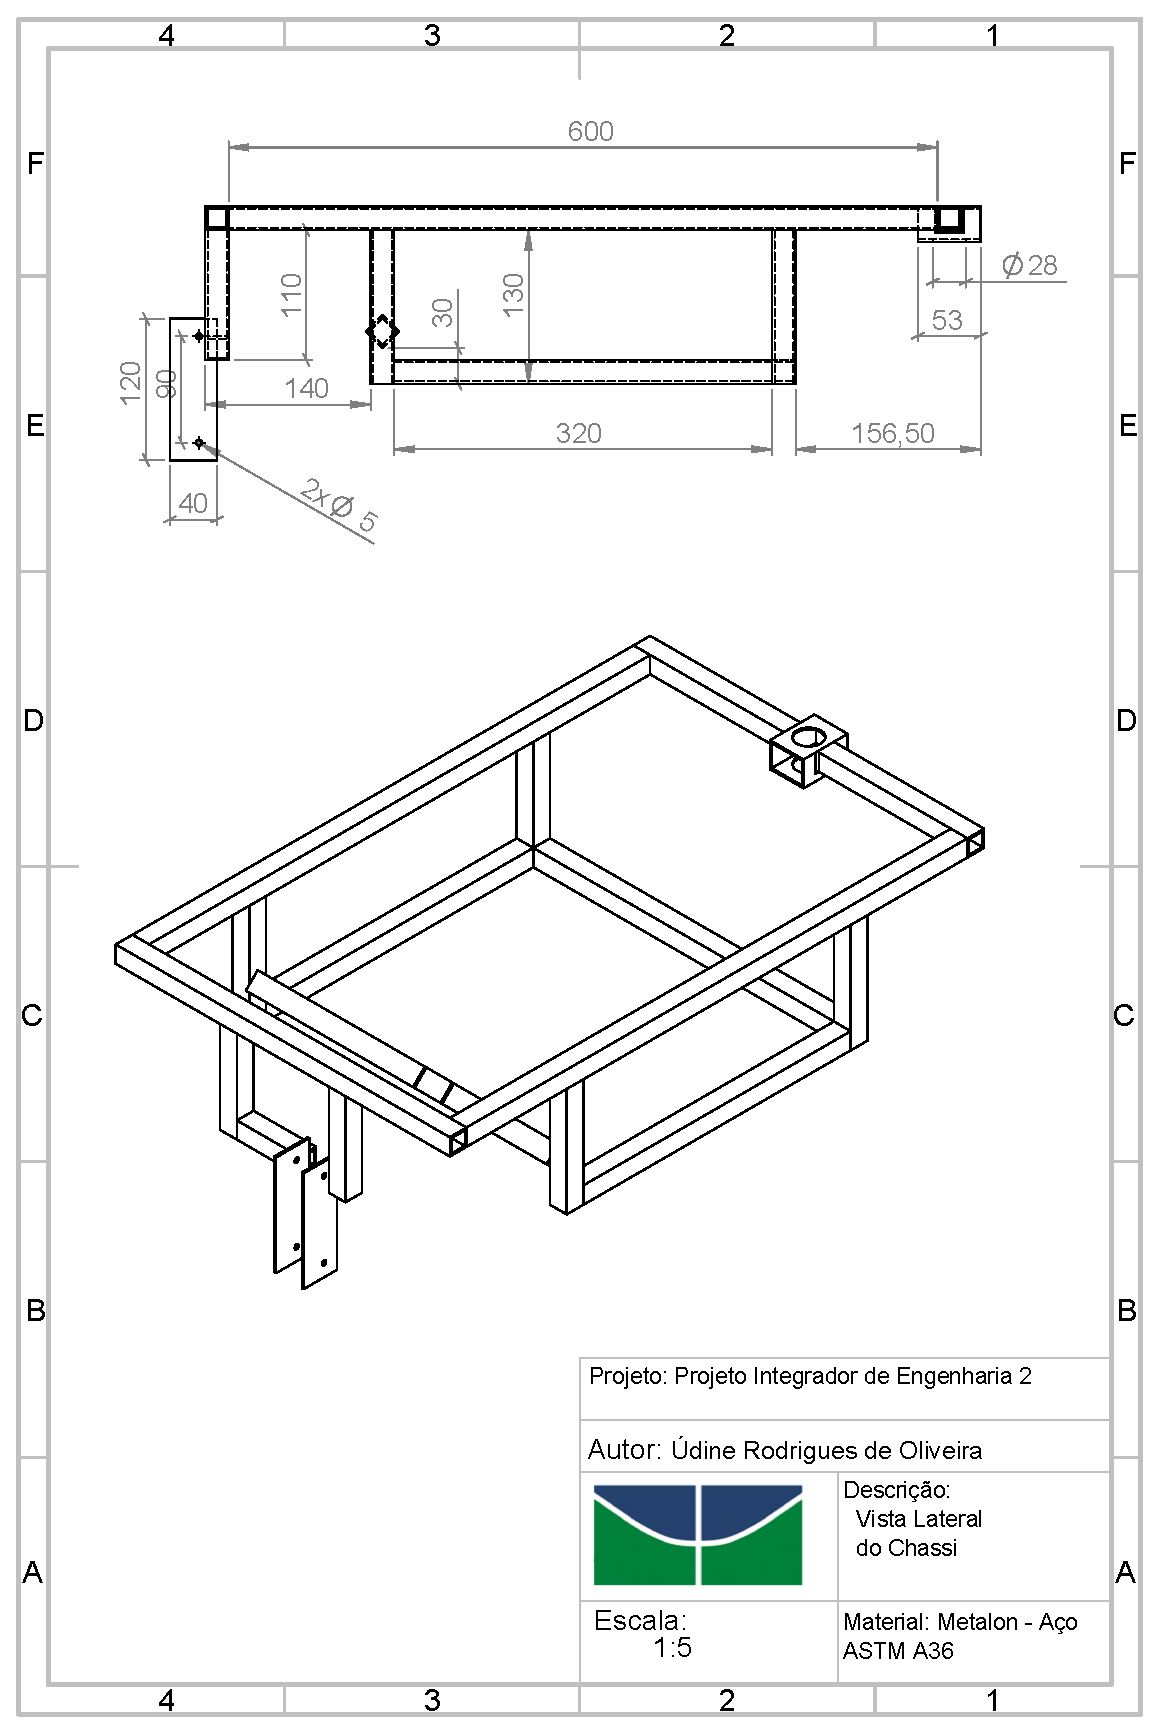
\includegraphics[width=\textwidth]{figuras/chassi_lateral.eps}
	\caption{Desenho técnico da lateral frontal do chassi}
\end{figure}

\begin{figure}[!htbp]
	\centering
	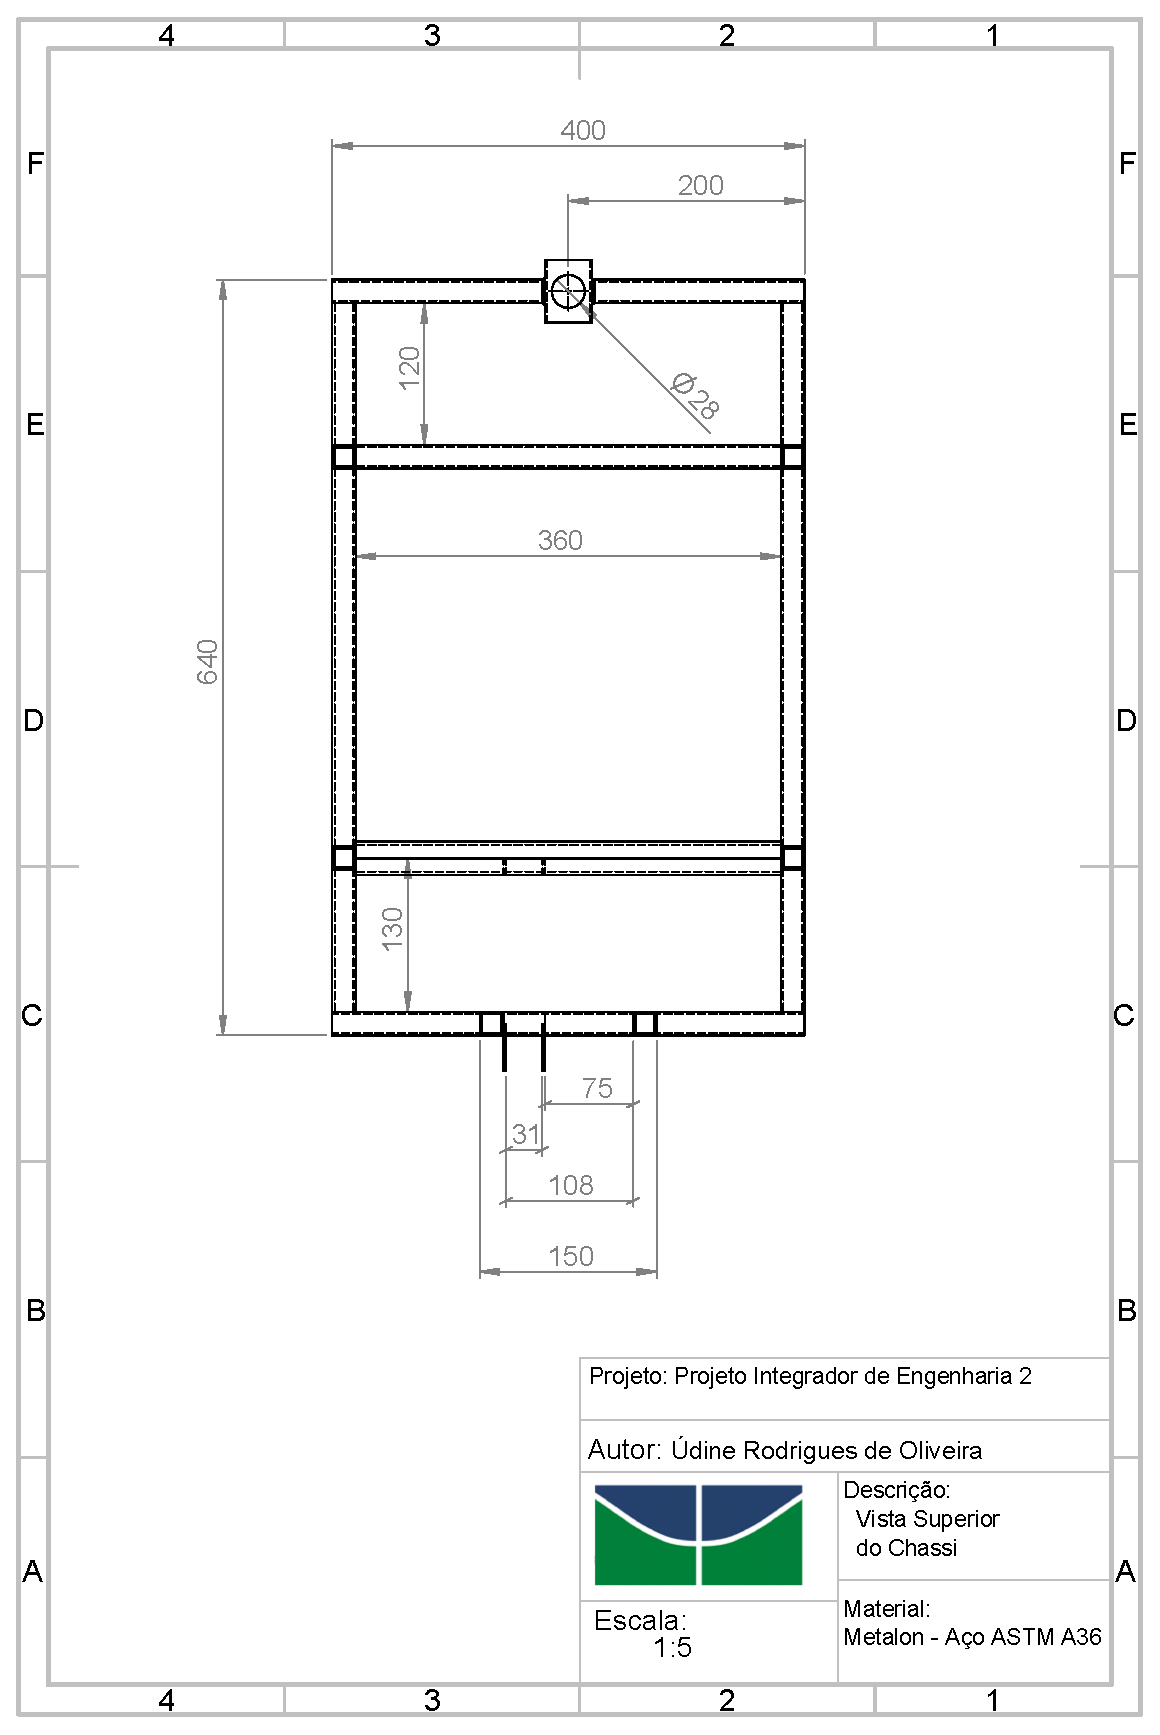
\includegraphics[width=\textwidth]{figuras/chassi_superior.eps}
	\caption{Desenho técnico da vista superior do chassi}
\end{figure}

\chapter{Manual de instruções}
\label{manuel}

Esse sistema é para a gerência do estado de sua plantação e configuação do carro autônomo para monitoramento de sua plantação de morango.

Ao acessar o sistema você irá se deparar com a página inicial onde terá quatro opções e uma ação, sendo que uma das quatro opções é o
manual que aqui se encontra.

\subsection{Configurações Gerais}

A primeira opção "Configurações Gerais", você irá se deparar com a opção de baixar os dados para que você obtenha as informações
coletadas pelo carro e também que você possa recuperar as medições feitas pelo veículo, se de alguma forma ocorrer perca dos dados
do seu sistema, com essa opção você recuperar esses dados do carro autônomo.

A outra opção você deverá antes de colocar o carro para trabalhar monitorando o campo, incluir as informações relacionado a quantidade
de fileiras ou cramalhões de sua plantação, para que o carro saiba quantas fileiras deve percorrer e quando deve ser sua parada.

A outra opção é relacionada a configuração de acesso ao carro autônomo, baseado nessa confoguração que ele consefuirá mandar os
dados que o mesmo precisa. A princípio essa opção já vem configurada, não precisando alterá-la, a não ser que você necessite
alterar o endereço de acesso ao carro.

\subsection{Minhas Medições}

A segunda opção "Minhas Medições" você poderá obter as informações coletadas pelo carro e com base neles, realizar a gerência
de sua plantação. Para que os dados apareçam, é necessário antes baixar as informações na opção de configurações gerais, e já
na opção Minha Medições, clicar no botão "Ler" para que o sistema leia os dados obtidos do carro e traga as informações.
Aqui você poderá verificar os dados principais que são umidade do solo, umidade do ar e temperatura do ar. Como observação a
umidade do solo ideal para plantações de morango deve estar entre 20 e 21 porcento.

\subsection{Calibração do sensor}

A terceira opção "Calibração do sensor" é onde você terá que antes de colocar o carro em ação para monitoração, calibrar
o sensor de umidade do solo do carro, pois caso não seja calibrado, os dados de umidade do seu solo, virão incorretas, e
isso pode acarretar prejuízo a sua plantação. Para calibração, será necessário seguir os seguintes passos:

\begin{itemize}
  \item Pegar uma amostra do seu solo com peso aproximado de 100 gramas.
  \item Fazer a secagem desta amostra com auxílio do microondas com potência entre 60 a 80 porcento.
  \item Esperar o tempo de 240 segundos ou 4 minutos exatos para estabilização da massa do solo.
  \item Pesar a amostra de solo seco e verificar se o mesmo está com 100 gramas.
  \item Caso dê um valor acima, retirar o excesso até atingir o valor de 100 gramas, caso não atinja esse valor, será necessário completar a amostra e repetir o processo de secagem.
  \item Pegar uma amostra de água destilada com peso de 5 gramas e umedecer a amostra.
  \item Misturar bem a amostra até obter uma amostra homogênea.
  \item Realizar a medição dessa amostra com o sensor de umidade e obter o valor.
  \item Os valores dos pesos do solo e da água passados são intencionais, pois com estes valoress, dará um valor de umidade de 5 porcento.
  \item O valor obtido da medida do sensor com o valor da umidade a 5 porcento indicará que para esta umidade o valor da medida do sensor é equivalente.
  \item Repetir esse procedimento para amostra de solo com 10, 15, 20, 25, 30, 40, 50 e 60 porcento, sendo estas porcentagens equivalentes ao valor do peso da água, e incluir esses valoes no sistema na parte de calibração do sistema.
\end{itemize}

\subsection{Iniciar Medições}

Esse botão você irá iniciar o carro depois de colocá-lo no ponto inicial para que realize as suas medições em sua plantação.



























\end{apendicesenv}
